\documentclass{beamer}

\usetheme{uhh}
\showtotalframenumber
\showuhhlogoeachframe
\showsections

\usepackage{amsmath}
\usepackage{graphicx}
\usepackage{color}
\DeclareMathOperator*{\argmin}{arg\,min}

\usepackage{listings}
\lstset{
  language=python
  }

\title{Deep Learning for Language and Speech - Seminar Projects}
\author{\underline{Benjamin Milde}, Prof. Dr. Chris Biemann}
\date[19.10.2017]{Oct 19, 2017}

\AtBeginSection[]
{
   %%%%% section title
   % This is how it would look like in Beamer:
   % \begin{frame}
   %     \frametitle{Overview}
   %     \tableofcontents[sections={2-3},currentsection,sectionstyle=show/hide,subsectionstyle=hide]
   % \end{frame}
  \begin{frame}[plain]
  \begin{tikzpicture}[overlay]
    \relax%
    \fill[blueuhh,opacity=1] (-10,-10)
    rectangle(\the\paperwidth,\the\paperheight);
  \end{tikzpicture}
   \begin{tikzpicture}[overlay]
    \relax%
    \fill[white,opacity=1] (-5,-1.2)
    rectangle(\the\paperwidth,0.5) node[pos=0.5,black]{\LARGE\insertsectionhead};
  \end{tikzpicture}
  \end{frame}

  %%%% add subsection to show navigation dots
  \subsection{}
}

\begin{document}

\maketitle

%\begin{frame}
%  \frametitle{Overview}
%
%  \begin{itemize}
%		\item Tensorflow Introduction / First session
%		\item Regression models
%		\item Neural tagger (DNN)
%		\item Implementing Word2Vec	
%		\item \textcolor{greyuhh}{Introduction to Tensorboard}
%		\item\textcolor{greyuhh}{Neural tagger (LSTM)}
%		\item \textcolor{greyuhh}{RNN language model (LSTM)}
%		\item \textcolor{greyuhh}{Maybe: Convolutions}
%	\end{itemize}
%\end{frame}

\section{Projects}

\begin{frame}
\frametitle{\#1 GermaNER tagger (1)}
\begin{itemize}
	\item German named entity recognition (organizations, names, places) with a twist - can you make the model compact?
	\item Dataset: https://github.com/tudarmstadt-lt/GermaNER
	\item Model accuracy vs. model size
	\item Many OOVs, will need a character model
	\item Might be used by LT projects e.g. new/s/leak (NetWork of Searchable Leaks), \url{https://www.inf.uni-hamburg.de/en/inst/ab/lt/resources/demos/new-s-leak.html}
 \end{itemize}
\end{frame}

\begin{frame}[fragile]
\frametitle{\#1 GermaNER tagger (2)}
\begin{tiny}
  \begin{verbatim}
	Schartau	B-PER
sagte	O
dem	O
"	O
Tagesspiegel	B-ORG
"	O
vom	O
Freitag	O
,	O
Fischer	B-PER
sei	O
"	O
... O

Firmengründer	O
Wolf	B-PER
Peter	I-PER
Bree	I-PER
arbeitete	O
Anfang	O
der	O
  \end{verbatim}
  \end{tiny}
\end{frame}

\begin{frame}[fragile]
\frametitle{\#2 Multilingual Emoji Prediction}
  \begin{itemize}
    \item SemEval-2018 task 2 competition
  	\item \url{https://competitions.codalab.org/competitions/17344#learn_the_details}  	
  \end{itemize}
  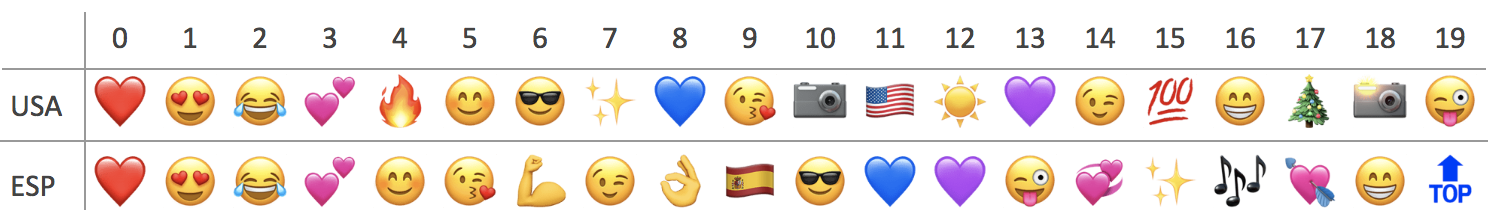
\includegraphics[width=0.8\textwidth]{semeval}
\end{frame}

\begin{frame}[fragile]
\frametitle{\#3 Irony detection in English tweets}
  \begin{itemize}
	\item SemEval-2018 task 3 competition
	\item \url{competitions.codalab.org/competitions/17468}
    \item Task a) binary classification:
    
\begin{verbatim} 
I just love when you test my patience!! #not
Had no sleep and have got school now #not happy
\end{verbatim}
	
	\item Task b)
	\item i) verbal irony realized through a polarity contrast, ii) verbal irony without such a polarity contrast (i.e., other verbal irony), iii) descriptions of situational irony, iv) non-irony. 
  \end{itemize}
\end{frame}

\begin{frame}[fragile]
\frametitle{\#4 One Million Posts Corpus}
  \begin{itemize}
\item DER STANDARD is an Austrian daily broadsheet newspaper. 
\item The data set contains a selection of user posts from the 12 month time span from 2015-06-01 to 2016-05-31. 
\item There are 11,773 labeled and 1,000,000 unlabeled posts in the data set.
\item Labels: \textbf{Sentiment} (negative/neutral/positive), \textbf{Off-Topic} (yes/no), \textbf{Inappropriate} (yes/no), \textbf{Discriminating} (yes/no)
  \end{itemize}

\end{frame}

\begin{frame}[fragile]
\frametitle{\#5 Common voice}
  \begin{itemize}
	\item Recently released speech dataset from mozilla
	\item 20000 speakers, some information about age, gender and accent available
	\item Predict those attributes (separately or together)

  \end{itemize}
  \begin{tiny}
  \begin{verbatim}
  ['cv-valid-dev/sample-004039.mp3', 'are you enjoying london',
   '1', '0', 'thirties', 'female', 'england', '']
['cv-valid-dev/sample-004040.mp3', 'they placed the symbols of the pilgrimage on the doors of their houses',
 '3', '0', 'sixties', 'female', 'us', '']
['cv-valid-dev/sample-004041.mp3', 'he could always go back to being a shepherd',
 '3', '0', '', '', '', '']
['cv-valid-dev/sample-004042.mp3', 'its lower end was still embedded',
 '6', '0', 'twenties', 'female', '', '']
['cv-valid-dev/sample-004043.mp3', "i'm going into the desert the man answered turning back to his reading",
 '1', '0', '', '', '', '']
['cv-valid-dev/sample-004044.mp3', 'as the sun rose the men began to beat the boy',
 '2', '0', 'thirties', 'male', 'australia', '']
['cv-valid-dev/sample-004045.mp3', 'i have to find a man who knows that universal language',
 '3', '0', 'thirties', 'male', 'us', '']
['cv-valid-dev/sample-004046.mp3', 'the picnic was ruined by a marching band',
 '1', '0', 'twenties', 'male', 'scotland', '']
  \end{verbatim}
    \end{tiny}
\end{frame}

\begin{frame}

\frametitle{\#6 Computational Paralinguistics}

 \begin{itemize}
 \item \url{http://emotion-research.net/sigs/speech-sig/is2017_compare.pdf}
 \item Normal speech vs. speaker has a cold challenge
 \item ALC corpus: \url{https://clarin.phonetik.uni-muenchen.de/BASRepository/}
 \item Intoxicated vs normal speech.
 \item Try transfer or multitask learning!
  \end{itemize}
  \end{frame}

\begin{frame}
\frametitle{\#7 G2P}
 \begin{itemize}
    \item abbreviate $\rightarrow$ AH B R IY V IY EY T
    \item Sequence to sequence models
 	\item Idea: Combine NLP and speech
 	\item Cmudict and speech samples (dict.cc)
 	\item \url{http://www.speech.cs.cmu.edu/cgi-bin/cmudict}
 	\item dict.cc
   \end{itemize}
\end{frame}

\begin{frame}
\frametitle{\#8 Your own idea here}
 \begin{itemize}
    \item As long as it is about text/speech
    \item And doable in a short time
   \end{itemize}
\end{frame}


%\section{Simple Optimization}
%
%% https://medium.com/@saxenarohan97/intro-to-tensorflow-solving-a-simple-regression-problem-e87b42fd4845
%% https://github.com/aymericdamien/TensorFlow-Examples/blob/master/examples/2_BasicModels/linear_regression.py
%\begin{frame}
%  \frametitle{Linear Regression}
%
%  \begin{itemize}
%  \item Given: $(x_1, y_1)$, \ldots, $(x_n,y_n)$
%  \item Goal: find $w$ and $b$ such that:
%    \begin{displaymath}
%      \argmin_{w, b} \frac{\sum^n_{i=1} (\hat{y}_i - y_i)^2}{n}
%    \end{displaymath}
%    where $\hat{y}_i = wx_i + b$.
%  \end{itemize}
%
%\end{frame}
%
%\begin{frame}[fragile]
%  \frametitle{Define model parameters}
%  Model: $\hat{y}_i = wx_i + b$
%
%\begin{lstlisting}
%w = tf.Variable(np.random.randn(), name="weight")
%b = tf.Variable(np.random.randn(), name="bias")
%\end{lstlisting}
%\end{frame}
%
%\begin{frame}[fragile]
%  \frametitle{Define the model}
%
%  \begin{displaymath}
%    \begin{pmatrix} \hat{y}_1\\\vdots\\\hat{y}_n\end{pmatrix} =
%    \begin{pmatrix} w\\\vdots\\w\end{pmatrix} *
%    \begin{pmatrix} \hat{x}_1\\\vdots\\\hat{x}_n\end{pmatrix} +
%    \begin{pmatrix} b\\\vdots\\b\end{pmatrix}
%  \end{displaymath}
%
%\begin{lstlisting}
%yhat = tf.add(tf.multiply(X, w), b)
%\end{lstlisting}
%
%{\footnotesize The scalars $w$ and $b$ are converted into vectors of the same
%  length as X (broadcast); \url{https://www.tensorflow.org/performance/xla/broadcasting}}
%
%\end{frame}
%
%\begin{frame}[fragile]
%  \frametitle{Define the loss}
%
%\begin{lstlisting}
%loss = tf.reduce_mean(tf.square(y - yhat))
%\end{lstlisting}
%
%\end{frame}
%
%
%\begin{frame}[fragile]
%  \frametitle{Optimization}
%
%\begin{lstlisting}
%epochs = 10
%optimizer = tf.train.GradientDescentOptimizer(
%    learning_rate).minimize(loss)
%
%with tf.Session() as sess:
%    ## initalize parameters
%    sess.run(tf.global_variables_initializer())
%
%    for i in list(range(epochs)):
%        ## run one epoch
%        sess.run(optimizer)
%        ## print result and loss
%        print(sess.run(yhat) + ' ' + sess.run(loss))
%\end{lstlisting}
%
%\end{frame}
%
%\begin{frame}[fragile]
%  \frametitle{Hands on: Simple optimization}
%
%  \begin{enumerate}
%  \item Do a linear regression to learn $y = 2x + 1$
%  \item Do a multiple linear regression with Boston housing prices
%  \end{enumerate}
%
%\begin{lstlisting}
%from sklearn.datasets import load_boston
%from sklearn.preprocessing import scale
%
%total_X, total_Y = load_boston(True)
%total_x = scale(total_x)
%\end{lstlisting}
%\end{frame}
%
%% https://www.tensorflow.org/tutorials/wide
%% https://github.com/aymericdamien/TensorFlow-Examples/blob/master/examples/2_BasicModels/logistic_regression.py
%\begin{frame}
%  \frametitle{Logistic regression}
%
%  TODO
%  tf.sigmoid
%
%\end{frame}
%
%\begin{frame}
%  \frametitle{Hands on: Regression model}
%
%  TODO: more complex example
%\end{frame}

\end{document}


%%% Local Variables:
%%% mode: latex
%%% TeX-engine: luatex
%%% End:
